
\chapter{Fonction inverse}
\competences{déterminer un domaine, dériver, étudier un signe, dresser un tableau de variations, représenter}
\section{Cours de référence}
La fonction inverse est définie par $f(x)=\dfrac1x$ sur $\R\setminus\{0\}$.

\begin{center}
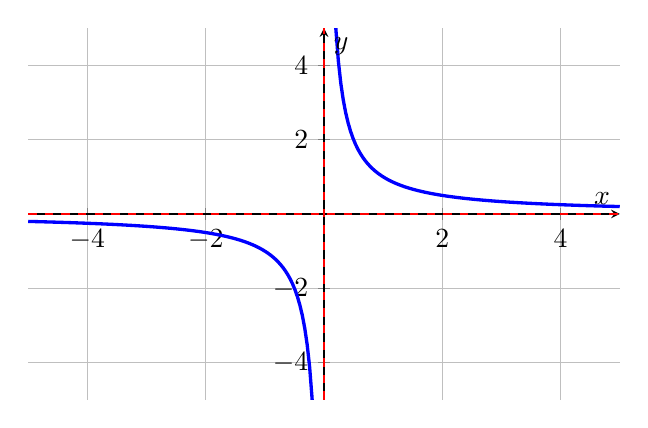
\begin{tikzpicture}
\begin{axis}[width=.75\textwidth,height=6.3cm,axis lines=middle,xmin=-5,xmax=5,ymin=-5,ymax=5,grid=major,xlabel={$x$},ylabel={$y$},unbounded coords=jump]
\addplot[Blue,very thick,samples=120,domain=-5:-.12]{1/x};
\addplot[Blue,very thick,samples=120,domain=.12:5]{1/x};
\addplot[Red,dashed,thick] coordinates {(0,-5)(0,5)};
\addplot[Red,dashed,thick] coordinates {(-5,0)(5,0)};
\end{axis}
\end{tikzpicture}
\end{center}

\begin{retenir}
$f'(x)=-\dfrac1{x^2}<0$ pour tout $x\neq0$. La fonction inverse est strictement décroissante sur chacun des intervalles $]-\infty,0[$ et $]0,+\infty[$. Les droites $x=0$ et $y=0$ sont des asymptotes.
\end{retenir}

\begin{erreur}
On ne peut pas écrire que la fonction inverse est décroissante « sur $\R\setminus\{0\}$ » sans préciser les deux intervalles. Par exemple $-1<1$ mais $f(-1)=-1<1=f(1)$, ce qui contreditrait la définition globale de la décroissance.
\end{erreur}

Pour une fonction $g(x)=P(x)+\dfrac{k}{x}$, on procède dans cet ordre : domaine ; dérivée ; mise au même dénominateur et factorisation ; signe de la dérivée ; variations ; limites ou comportement aux bornes ; points utiles ; représentation.

\begin{exemple}
Sur $]0,+\infty[$, $g(x)=x+\dfrac4x$ vérifie $g'(x)=1-\dfrac4{x^2}=\dfrac{(x-2)(x+2)}{x^2}$. Le dénominateur est positif ; $g'$ est négative sur $]0,2[$ puis positive sur $]2,+\infty[$. La fonction admet un minimum $g(2)=4$.
\end{exemple}

\sessionheader{23}{15/12/2026}{B : 2 h -- C : 1 h}{Définition et courbe de la fonction inverse}{Fonction inverse}
\begin{objectifs}\begin{itemize}\item Déterminer le domaine.\item Construire la courbe.\item Utiliser les symétries.\end{itemize}\end{objectifs}
\begin{automatismes}\begin{enumerate}\item Réduire $3x+5-x+2$. \rep{$2x+7$}\item Donner la valeur interdite de $\dfrac{x+1}{x}$. \rep{$x=0$}\item Calculer $\dfrac1{5}$ et $\dfrac1{-5}$. \rep{$\dfrac1{5}$ et $-\dfrac1{5}$}\item Dériver $3x^2-5x+1$. \rep{$6x-5$}\item Résoudre $(x-2)(x+1)=0$. \rep{$x=-1$ ou $x=2$}\end{enumerate}\end{automatismes}
\begin{prerequis}Relire la dernière trace écrite et savoir effectuer les calculs élémentaires mobilisés aujourd'hui. Avant l'activité, faire reformuler les mots-clés : déterminer le domaine et construire la courbe.\end{prerequis}

\begin{activite}
Calculer $\dfrac1x$ pour $x=-4,-2,-1,-\dfrac12,\dfrac12,1,2,4$. Placer les points et décrire les symétries. Pourquoi $x=0$ est-il absent ?
\begin{center}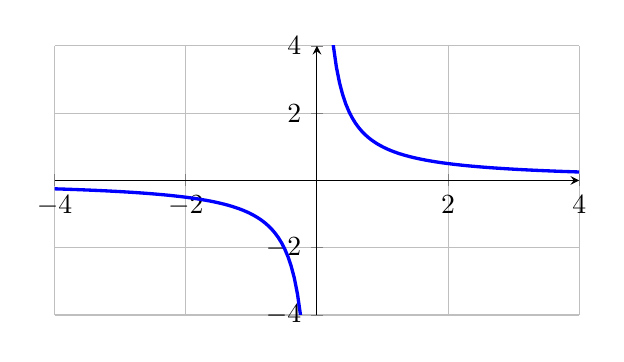
\begin{tikzpicture}\begin{axis}[width=.68\textwidth,height=5cm,axis lines=middle,xmin=-4,xmax=4,ymin=-4,ymax=4,grid=major]\addplot[Blue,very thick,samples=80,domain=-4:-.15]{1/x};\addplot[Blue,very thick,samples=80,domain=.15:4]{1/x};\end{axis}\end{tikzpicture}\end{center}
\end{activite}
\enseignant{Les valeurs sont respectivement $-\frac14,-\frac12,-1,-2,2,1,\frac12,\frac14$. Le domaine exclut $0$ ; la courbe est symétrique par rapport à l'origine. Faire verbaliser la donnée qui déclenche le choix de méthode.}

\begin{traceecrite}La fonction inverse est $f(x)=\dfrac1x$ sur $\R\setminus\{0\}$. Sa courbe est une hyperbole symétrique par rapport à l'origine.\end{traceecrite}

\begin{exemple}
Reprendre les données de l'activité et rédiger la solution dans l'ordre : définition des objets, propriété utilisée, calcul exact ou approché, puis phrase de réponse. La réponse modèle figure dans l'édition enseignant.
\end{exemple}
\enseignant{Les valeurs sont respectivement $-\frac14,-\frac12,-1,-2,2,1,\frac12,\frac14$. Le domaine exclut $0$ ; la courbe est symétrique par rapport à l'origine.}

\begin{exercice}[-- essentiel]
\begin{enumerate}\item Donner le domaine et les asymptotes de $f(x)=5+\dfrac{7}x$.\item Calculer $f'(x)$ et étudier son signe.\item Étudier sur $]0,+\infty[$ la fonction $g(x)=x+\dfrac{25}x$.\end{enumerate}
\end{exercice}
\enseignant{Le domaine est $\R\setminus\{0\}$ ; asymptotes $x=0$ et $y=5$. $f'(x)=-\dfrac{7}{x^2}<0$. Pour $g$, $g'(x)=1-\dfrac{25}{x^2}$ et le minimum est atteint en $x=5$, de valeur $10$.}

\manuelref{Calao, cours p. 88--93 ; exercices p. 94, n° 1 à 5}
\ExoSession{23}

\begin{dm}Reprendre l'exercice d'entraînement 2 avec les données suivantes : remplacer la donnée initiale par $235$ et le taux ou la raison par $7$. Rédiger en quatre lignes : données, formule, calcul, conclusion.\end{dm}
\enseignant{La correction dépend de l'exercice repris. Vérifier surtout la cohérence du modèle, le nombre d'itérations, l'arrondi et la phrase de conclusion.}

\begin{sortie}Sur une demi-feuille : écrire la règle principale de la séance, traiter un exemple très court et indiquer son degré de confiance de 1 à 4. Question(s) essentielle(s) du jour : 1, 2 et 3.\end{sortie}

\ifprof
\begin{methode}
\textbf{Conduite en 1 h :} 7 min d'automatismes ; 10 min de mise en commun et trace ; 28 min d'exercices essentiels ; 5 min de correction ; 3 min de billet de sortie.\\
\textbf{Conduite en 2 h :} ajouter 20 min de recherche de l'activité, 20 min d'institutionnalisation, un second exercice autonome et 10 min de correction comparée.\\
\textbf{Différenciation :} fournir aux élèves fragiles une fiche à quatre cases (données, modèle, calcul, conclusion). Demander aux élèves rapides de produire un contre-exemple, une justification ou une seconde méthode.
\end{methode}
\fi
\sessionheader{24}{17/12/2026}{B : 1 h -- C : 2 h}{Comportement aux bornes et asymptotes}{Fonction inverse}
\begin{objectifs}\begin{itemize}\item Décrire le comportement aux bornes.\item Identifier les asymptotes.\item Lire une représentation.\end{itemize}\end{objectifs}
\begin{automatismes}\begin{enumerate}\item Calculer $5\,\%$ de $120$. \rep{$6$}\item Calculer $\dfrac1{6}$ et $\dfrac1{-6}$. \rep{$\dfrac1{6}$ et $-\dfrac1{6}$}\item Dériver $3x^2-5x+1$. \rep{$6x-5$}\item Résoudre $(x-2)(x+1)=0$. \rep{$x=-1$ ou $x=2$}\item Donner la valeur interdite de $\dfrac{x+1}{x}$. \rep{$x=0$}\end{enumerate}\end{automatismes}
\begin{prerequis}Relire la dernière trace écrite et savoir effectuer les calculs élémentaires mobilisés aujourd'hui. Avant l'activité, faire reformuler les mots-clés : décrire le comportement aux bornes et identifier les asymptotes.\end{prerequis}

\begin{activite}
À l'aide d'un tableau de valeurs près de $0$ et pour de grandes valeurs de $|x|$, décrire $\dfrac1x$. Traduire chaque comportement par une asymptote et par une phrase.
\begin{center}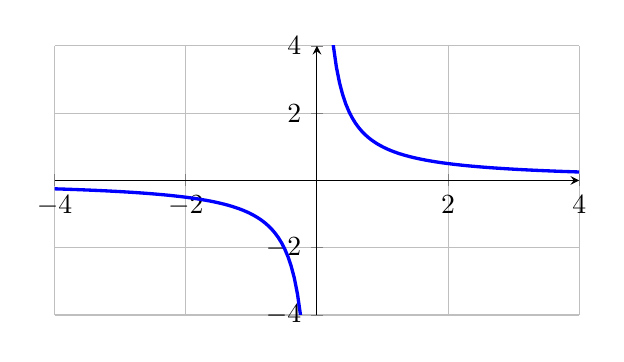
\begin{tikzpicture}\begin{axis}[width=.68\textwidth,height=5cm,axis lines=middle,xmin=-4,xmax=4,ymin=-4,ymax=4,grid=major]\addplot[Blue,very thick,samples=80,domain=-4:-.15]{1/x};\addplot[Blue,very thick,samples=80,domain=.15:4]{1/x};\end{axis}\end{tikzpicture}\end{center}
\end{activite}
\enseignant{Près de $0$, les valeurs deviennent très grandes en valeur absolue : asymptote $x=0$. Quand $|x|$ grandit, $\dfrac1x$ se rapproche de $0$ : asymptote $y=0$. Faire verbaliser la donnée qui déclenche le choix de méthode.}

\begin{traceecrite}Pour $f(x)=\dfrac1x$, $x=0$ est asymptote verticale et $y=0$ asymptote horizontale. Les branches s'en approchent sans les couper.\end{traceecrite}

\begin{exemple}
Reprendre les données de l'activité et rédiger la solution dans l'ordre : définition des objets, propriété utilisée, calcul exact ou approché, puis phrase de réponse. La réponse modèle figure dans l'édition enseignant.
\end{exemple}
\enseignant{Près de $0$, les valeurs deviennent très grandes en valeur absolue : asymptote $x=0$. Quand $|x|$ grandit, $\dfrac1x$ se rapproche de $0$ : asymptote $y=0$.}

\begin{exercice}[-- essentiel]
\begin{enumerate}\item Donner le domaine et les asymptotes de $f(x)=6+\dfrac{8}x$.\item Calculer $f'(x)$ et étudier son signe.\item Étudier sur $]0,+\infty[$ la fonction $g(x)=x+\dfrac{36}x$.\end{enumerate}
\end{exercice}
\enseignant{Le domaine est $\R\setminus\{0\}$ ; asymptotes $x=0$ et $y=6$. $f'(x)=-\dfrac{8}{x^2}<0$. Pour $g$, $g'(x)=1-\dfrac{36}{x^2}$ et le minimum est atteint en $x=6$, de valeur $12$.}

\manuelref{Calao, cours p. 88--93 ; exercices p. 94, n° 4 à 9}
\ExoSession{24}

\begin{dm}Reprendre l'exercice d'entraînement 3 avec les données suivantes : remplacer la donnée initiale par $240$ et le taux ou la raison par $2$. Rédiger en quatre lignes : données, formule, calcul, conclusion.\end{dm}
\enseignant{La correction dépend de l'exercice repris. Vérifier surtout la cohérence du modèle, le nombre d'itérations, l'arrondi et la phrase de conclusion.}

\begin{sortie}Sur une demi-feuille : écrire la règle principale de la séance, traiter un exemple très court et indiquer son degré de confiance de 1 à 4. Question(s) essentielle(s) du jour : 1 et 2.\end{sortie}

\ifprof
\begin{methode}
\textbf{Conduite en 1 h :} 7 min d'automatismes ; 10 min de mise en commun et trace ; 28 min d'exercices essentiels ; 5 min de correction ; 3 min de billet de sortie.\\
\textbf{Conduite en 2 h :} ajouter 20 min de recherche de l'activité, 20 min d'institutionnalisation, un second exercice autonome et 10 min de correction comparée.\\
\textbf{Différenciation :} fournir aux élèves fragiles une fiche à quatre cases (données, modèle, calcul, conclusion). Demander aux élèves rapides de produire un contre-exemple, une justification ou une seconde méthode.
\end{methode}
\fi
\sessionheader{25}{05/01/2027}{B : 2 h -- C : 1 h}{Dérivée et sens de variation}{Fonction inverse}
\begin{objectifs}\begin{itemize}\item Dériver la fonction inverse.\item Justifier les variations.\item Dresser un tableau.\end{itemize}\end{objectifs}
\begin{automatismes}\begin{enumerate}\item Écrire le coefficient multiplicateur d'une hausse de $10\,\%$. \rep{$1+\dfrac{10}{100}=1,10$}\item Dériver $3x^2-5x+1$. \rep{$6x-5$}\item Résoudre $(x-2)(x+1)=0$. \rep{$x=-1$ ou $x=2$}\item Donner la valeur interdite de $\dfrac{x+1}{x}$. \rep{$x=0$}\item Calculer $\dfrac1{7}$ et $\dfrac1{-7}$. \rep{$\dfrac1{7}$ et $-\dfrac1{7}$}\end{enumerate}\end{automatismes}
\begin{prerequis}Relire la dernière trace écrite et savoir effectuer les calculs élémentaires mobilisés aujourd'hui. Avant l'activité, faire reformuler les mots-clés : dériver la fonction inverse et justifier les variations.\end{prerequis}

\begin{activite}
À partir du taux d'accroissement de $f(x)=\dfrac1x$, retrouver $f'(x)=-\dfrac1{x^2}$. Étudier son signe et vérifier la cohérence avec le graphique.

\end{activite}
\enseignant{Le carré $x^2$ est positif pour $x\neq0$, donc la dérivée est strictement négative sur chacun des intervalles du domaine. Faire verbaliser la donnée qui déclenche le choix de méthode.}

\begin{traceecrite}Pour $x\neq0$, $f'(x)=-\dfrac1{x^2}<0$. La fonction inverse décroît sur chacun des intervalles $]-\infty,0[$ et $]0,+\infty[$.\end{traceecrite}

\begin{exemple}
Reprendre les données de l'activité et rédiger la solution dans l'ordre : définition des objets, propriété utilisée, calcul exact ou approché, puis phrase de réponse. La réponse modèle figure dans l'édition enseignant.
\end{exemple}
\enseignant{Le carré $x^2$ est positif pour $x\neq0$, donc la dérivée est strictement négative sur chacun des intervalles du domaine.}

\begin{exercice}[-- essentiel]
\begin{enumerate}\item Donner le domaine et les asymptotes de $f(x)=2+\dfrac{4}x$.\item Calculer $f'(x)$ et étudier son signe.\item Étudier sur $]0,+\infty[$ la fonction $g(x)=x+\dfrac{4}x$.\end{enumerate}
\end{exercice}
\enseignant{Le domaine est $\R\setminus\{0\}$ ; asymptotes $x=0$ et $y=2$. $f'(x)=-\dfrac{4}{x^2}<0$. Pour $g$, $g'(x)=1-\dfrac{4}{x^2}$ et le minimum est atteint en $x=2$, de valeur $4$.}

\manuelref{Calao, cours p. 89--93 ; exercices p. 94, n° 1 à 3, puis p. 96, n° 10 à 13}
\ExoSession{25}

\begin{dm}Reprendre l'exercice d'entraînement 2 avec les données suivantes : remplacer la donnée initiale par $245$ et le taux ou la raison par $3$. Rédiger en quatre lignes : données, formule, calcul, conclusion.\end{dm}
\enseignant{La correction dépend de l'exercice repris. Vérifier surtout la cohérence du modèle, le nombre d'itérations, l'arrondi et la phrase de conclusion.}

\begin{sortie}Sur une demi-feuille : écrire la règle principale de la séance, traiter un exemple très court et indiquer son degré de confiance de 1 à 4. Question(s) essentielle(s) du jour : 1, 2 et 3.\end{sortie}

\ifprof
\begin{methode}
\textbf{Conduite en 1 h :} 7 min d'automatismes ; 10 min de mise en commun et trace ; 28 min d'exercices essentiels ; 5 min de correction ; 3 min de billet de sortie.\\
\textbf{Conduite en 2 h :} ajouter 20 min de recherche de l'activité, 20 min d'institutionnalisation, un second exercice autonome et 10 min de correction comparée.\\
\textbf{Différenciation :} fournir aux élèves fragiles une fiche à quatre cases (données, modèle, calcul, conclusion). Demander aux élèves rapides de produire un contre-exemple, une justification ou une seconde méthode.
\end{methode}
\fi
\sessionheader{26}{07/01/2027}{B : 1 h -- C : 2 h}{Combinaisons avec des fonctions polynomiales}{Fonction inverse}
\begin{objectifs}\begin{itemize}\item Dériver une combinaison.\item Réduire une expression.\item Organiser une étude.\end{itemize}\end{objectifs}
\begin{automatismes}\begin{enumerate}\item Réduire $3x+8-x+2$. \rep{$2x+10$}\item Résoudre $(x-2)(x+1)=0$. \rep{$x=-1$ ou $x=2$}\item Donner la valeur interdite de $\dfrac{x+1}{x}$. \rep{$x=0$}\item Calculer $\dfrac1{8}$ et $\dfrac1{-8}$. \rep{$\dfrac1{8}$ et $-\dfrac1{8}$}\item Dériver $3x^2-5x+1$. \rep{$6x-5$}\end{enumerate}\end{automatismes}
\begin{prerequis}Relire la dernière trace écrite et savoir effectuer les calculs élémentaires mobilisés aujourd'hui. Avant l'activité, faire reformuler les mots-clés : dériver une combinaison et réduire une expression.\end{prerequis}

\begin{activite}
Une entreprise produit $x>0$ centaines d'objets et son coût moyen est $C(x)=2x+30+\dfrac{200}{x}$. Calculer $C'(x)$, factoriser son numérateur et chercher le niveau de production minimisant le coût moyen.

\end{activite}
\enseignant{$C'(x)=2-\dfrac{200}{x^2}=\dfrac{2(x-10)(x+10)}{x^2}$. Le minimum est atteint pour $x=10$, soit $1\,000$ objets. Faire verbaliser la donnée qui déclenche le choix de méthode.}

\begin{traceecrite}Pour étudier $P(x)+\dfrac{k}{x}$, déterminer le domaine, calculer la dérivée, réduire au même dénominateur, étudier son signe puis dresser les variations.\end{traceecrite}

\begin{exemple}
Reprendre les données de l'activité et rédiger la solution dans l'ordre : définition des objets, propriété utilisée, calcul exact ou approché, puis phrase de réponse. La réponse modèle figure dans l'édition enseignant.
\end{exemple}
\enseignant{$C'(x)=2-\dfrac{200}{x^2}=\dfrac{2(x-10)(x+10)}{x^2}$. Le minimum est atteint pour $x=10$, soit $1\,000$ objets.}

\begin{exercice}[-- essentiel]
\begin{enumerate}\item Donner le domaine et les asymptotes de $f(x)=3+\dfrac{5}x$.\item Calculer $f'(x)$ et étudier son signe.\item Étudier sur $]0,+\infty[$ la fonction $g(x)=x+\dfrac{9}x$.\end{enumerate}
\end{exercice}
\enseignant{Le domaine est $\R\setminus\{0\}$ ; asymptotes $x=0$ et $y=3$. $f'(x)=-\dfrac{5}{x^2}<0$. Pour $g$, $g'(x)=1-\dfrac{9}{x^2}$ et le minimum est atteint en $x=3$, de valeur $6$.}

\manuelref{Calao, p. 96, n° 14 à 21}
\ExoSession{26}

\begin{dm}Reprendre l'exercice d'entraînement 3 avec les données suivantes : remplacer la donnée initiale par $250$ et le taux ou la raison par $4$. Rédiger en quatre lignes : données, formule, calcul, conclusion.\end{dm}
\enseignant{La correction dépend de l'exercice repris. Vérifier surtout la cohérence du modèle, le nombre d'itérations, l'arrondi et la phrase de conclusion.}

\begin{sortie}Sur une demi-feuille : écrire la règle principale de la séance, traiter un exemple très court et indiquer son degré de confiance de 1 à 4. Question(s) essentielle(s) du jour : 1 et 2.\end{sortie}

\ifprof
\begin{methode}
\textbf{Conduite en 1 h :} 7 min d'automatismes ; 10 min de mise en commun et trace ; 28 min d'exercices essentiels ; 5 min de correction ; 3 min de billet de sortie.\\
\textbf{Conduite en 2 h :} ajouter 20 min de recherche de l'activité, 20 min d'institutionnalisation, un second exercice autonome et 10 min de correction comparée.\\
\textbf{Différenciation :} fournir aux élèves fragiles une fiche à quatre cases (données, modèle, calcul, conclusion). Demander aux élèves rapides de produire un contre-exemple, une justification ou une seconde méthode.
\end{methode}
\fi
\sessionheader{27}{12/01/2027}{B : 2 h -- C : 1 h}{Signe et factorisation}{Fonction inverse}
\begin{objectifs}\begin{itemize}\item Factoriser.\item Construire un tableau de signes.\item Respecter les valeurs interdites.\end{itemize}\end{objectifs}
\begin{automatismes}\begin{enumerate}\item Calculer $20\,\%$ de $180$. \rep{$36$}\item Donner la valeur interdite de $\dfrac{x+1}{x}$. \rep{$x=0$}\item Calculer $\dfrac1{9}$ et $\dfrac1{-9}$. \rep{$\dfrac1{9}$ et $-\dfrac1{9}$}\item Dériver $3x^2-5x+1$. \rep{$6x-5$}\item Résoudre $(x-2)(x+1)=0$. \rep{$x=-1$ ou $x=2$}\end{enumerate}\end{automatismes}
\begin{prerequis}Relire la dernière trace écrite et savoir effectuer les calculs élémentaires mobilisés aujourd'hui. Avant l'activité, faire reformuler les mots-clés : factoriser et construire un tableau de signes.\end{prerequis}

\begin{activite}
Étudier le signe de $\dfrac{(x-2)(x+3)}x$. Construire le tableau avec les trois valeurs critiques, distinguer zéro et valeur interdite, puis résoudre l'inéquation $\dfrac{(x-2)(x+3)}x\geq0$.

\end{activite}
\enseignant{Les valeurs critiques sont $-3,0,2$. La solution est $[-3,0[\cup[2,+\infty[$. Faire verbaliser la donnée qui déclenche le choix de méthode.}

\begin{traceecrite}Dans un quotient, le signe dépend du numérateur et du dénominateur. Les valeurs interdites sont exclues du tableau, même si un facteur se simplifie formellement.\end{traceecrite}

\begin{exemple}
Reprendre les données de l'activité et rédiger la solution dans l'ordre : définition des objets, propriété utilisée, calcul exact ou approché, puis phrase de réponse. La réponse modèle figure dans l'édition enseignant.
\end{exemple}
\enseignant{Les valeurs critiques sont $-3,0,2$. La solution est $[-3,0[\cup[2,+\infty[$.}

\begin{exercice}[-- essentiel]
\begin{enumerate}\item Donner le domaine et les asymptotes de $f(x)=4+\dfrac{6}x$.\item Calculer $f'(x)$ et étudier son signe.\item Étudier sur $]0,+\infty[$ la fonction $g(x)=x+\dfrac{16}x$.\end{enumerate}
\end{exercice}
\enseignant{Le domaine est $\R\setminus\{0\}$ ; asymptotes $x=0$ et $y=4$. $f'(x)=-\dfrac{6}{x^2}<0$. Pour $g$, $g'(x)=1-\dfrac{16}{x^2}$ et le minimum est atteint en $x=4$, de valeur $8$.}

\manuelref{Calao, p. 96 à 101}
\ExoSession{27}

\begin{dm}Reprendre l'exercice d'entraînement 2 avec les données suivantes : remplacer la donnée initiale par $255$ et le taux ou la raison par $5$. Rédiger en quatre lignes : données, formule, calcul, conclusion.\end{dm}
\enseignant{La correction dépend de l'exercice repris. Vérifier surtout la cohérence du modèle, le nombre d'itérations, l'arrondi et la phrase de conclusion.}

\begin{sortie}Sur une demi-feuille : écrire la règle principale de la séance, traiter un exemple très court et indiquer son degré de confiance de 1 à 4. Question(s) essentielle(s) du jour : 1, 2 et 3.\end{sortie}

\ifprof
\begin{methode}
\textbf{Conduite en 1 h :} 7 min d'automatismes ; 10 min de mise en commun et trace ; 28 min d'exercices essentiels ; 5 min de correction ; 3 min de billet de sortie.\\
\textbf{Conduite en 2 h :} ajouter 20 min de recherche de l'activité, 20 min d'institutionnalisation, un second exercice autonome et 10 min de correction comparée.\\
\textbf{Différenciation :} fournir aux élèves fragiles une fiche à quatre cases (données, modèle, calcul, conclusion). Demander aux élèves rapides de produire un contre-exemple, une justification ou une seconde méthode.
\end{methode}
\fi
\sessionheader{28}{14/01/2027}{B : 1 h -- C : 2 h}{Dérivées de polynômes de degré au plus 3}{Fonction inverse}
\begin{objectifs}\begin{itemize}\item Dériver un polynôme.\item Étudier une dérivée.\item Déduire des variations.\end{itemize}\end{objectifs}
\begin{automatismes}\begin{enumerate}\item Écrire le coefficient multiplicateur d'une hausse de $25\,\%$. \rep{$1+\dfrac{25}{100}=1,25$}\item Calculer $\dfrac1{3}$ et $\dfrac1{-3}$. \rep{$\dfrac1{3}$ et $-\dfrac1{3}$}\item Dériver $3x^2-5x+1$. \rep{$6x-5$}\item Résoudre $(x-2)(x+1)=0$. \rep{$x=-1$ ou $x=2$}\item Donner la valeur interdite de $\dfrac{x+1}{x}$. \rep{$x=0$}\end{enumerate}\end{automatismes}
\begin{prerequis}Relire la dernière trace écrite et savoir effectuer les calculs élémentaires mobilisés aujourd'hui. Avant l'activité, faire reformuler les mots-clés : dériver un polynôme et étudier une dérivée.\end{prerequis}

\begin{activite}
Pour $f(x)=2x^3-3x^2-12x+5$, calculer $f'(x)$, factoriser, étudier son signe et en déduire les variations de $f$.

\end{activite}
\enseignant{$f'(x)=6x^2-6x-12=6(x-2)(x+1)$. La fonction croît sur $]-\infty,-1]$, décroît sur $[-1,2]$, puis croît. Faire verbaliser la donnée qui déclenche le choix de méthode.}

\begin{traceecrite}$(ax^3+bx^2+cx+d)'=3ax^2+2bx+c$. Le signe de la dérivée donne le sens de variation de la fonction.\end{traceecrite}

\begin{exemple}
Reprendre les données de l'activité et rédiger la solution dans l'ordre : définition des objets, propriété utilisée, calcul exact ou approché, puis phrase de réponse. La réponse modèle figure dans l'édition enseignant.
\end{exemple}
\enseignant{$f'(x)=6x^2-6x-12=6(x-2)(x+1)$. La fonction croît sur $]-\infty,-1]$, décroît sur $[-1,2]$, puis croît.}

\begin{exercice}[-- essentiel]
\begin{enumerate}\item Donner le domaine et les asymptotes de $f(x)=5+\dfrac{7}x$.\item Calculer $f'(x)$ et étudier son signe.\item Étudier sur $]0,+\infty[$ la fonction $g(x)=x+\dfrac{25}x$.\end{enumerate}
\end{exercice}
\enseignant{Le domaine est $\R\setminus\{0\}$ ; asymptotes $x=0$ et $y=5$. $f'(x)=-\dfrac{7}{x^2}<0$. Pour $g$, $g'(x)=1-\dfrac{25}{x^2}$ et le minimum est atteint en $x=5$, de valeur $10$.}

\manuelref{Calao, p. 94 à 96}
\ExoSession{28}

\begin{dm}Reprendre l'exercice d'entraînement 3 avec les données suivantes : remplacer la donnée initiale par $260$ et le taux ou la raison par $6$. Rédiger en quatre lignes : données, formule, calcul, conclusion.\end{dm}
\enseignant{La correction dépend de l'exercice repris. Vérifier surtout la cohérence du modèle, le nombre d'itérations, l'arrondi et la phrase de conclusion.}

\begin{sortie}Sur une demi-feuille : écrire la règle principale de la séance, traiter un exemple très court et indiquer son degré de confiance de 1 à 4. Question(s) essentielle(s) du jour : 1 et 2.\end{sortie}

\ifprof
\begin{methode}
\textbf{Conduite en 1 h :} 7 min d'automatismes ; 10 min de mise en commun et trace ; 28 min d'exercices essentiels ; 5 min de correction ; 3 min de billet de sortie.\\
\textbf{Conduite en 2 h :} ajouter 20 min de recherche de l'activité, 20 min d'institutionnalisation, un second exercice autonome et 10 min de correction comparée.\\
\textbf{Différenciation :} fournir aux élèves fragiles une fiche à quatre cases (données, modèle, calcul, conclusion). Demander aux élèves rapides de produire un contre-exemple, une justification ou une seconde méthode.
\end{methode}
\fi
\sessionheader{29}{19/01/2027}{B : 2 h -- C : 1 h}{Étude complète et représentation}{Fonction inverse}
\begin{objectifs}\begin{itemize}\item Mener une étude complète.\item Tracer une courbe cohérente.\item Interpréter un extremum.\end{itemize}\end{objectifs}
\begin{automatismes}\begin{enumerate}\item Réduire $3x+4-x+2$. \rep{$2x+6$}\item Dériver $3x^2-5x+1$. \rep{$6x-5$}\item Résoudre $(x-2)(x+1)=0$. \rep{$x=-1$ ou $x=2$}\item Donner la valeur interdite de $\dfrac{x+1}{x}$. \rep{$x=0$}\item Calculer $\dfrac1{4}$ et $\dfrac1{-4}$. \rep{$\dfrac1{4}$ et $-\dfrac1{4}$}\end{enumerate}\end{automatismes}
\begin{prerequis}Relire la dernière trace écrite et savoir effectuer les calculs élémentaires mobilisés aujourd'hui. Avant l'activité, faire reformuler les mots-clés : mener une étude complète et tracer une courbe cohérente.\end{prerequis}

\begin{activite}
Étudier complètement $g(x)=x+\dfrac9x$ sur $]0,+\infty[$ : domaine, dérivée, signe, variations, minimum, comportement aux bornes et esquisse.
\begin{center}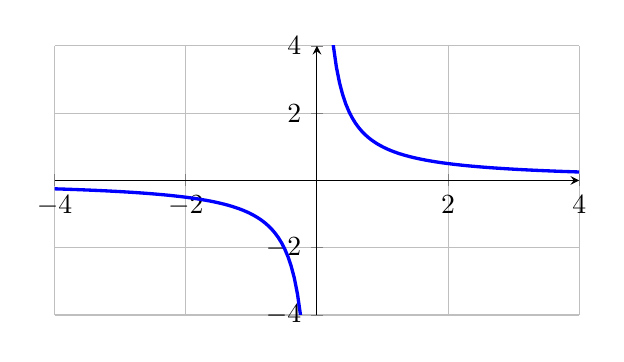
\begin{tikzpicture}\begin{axis}[width=.68\textwidth,height=5cm,axis lines=middle,xmin=-4,xmax=4,ymin=-4,ymax=4,grid=major]\addplot[Blue,very thick,samples=80,domain=-4:-.15]{1/x};\addplot[Blue,very thick,samples=80,domain=.15:4]{1/x};\end{axis}\end{tikzpicture}\end{center}
\end{activite}
\enseignant{$g'(x)=\dfrac{(x-3)(x+3)}{x^2}$ ; minimum $g(3)=6$ ; $g(x)$ tend vers $+\infty$ en $0^+$ et en $+\infty$. Faire verbaliser la donnée qui déclenche le choix de méthode.}

\begin{traceecrite}Une étude complète comporte : domaine, dérivée, signe, variations, limites ou comportement aux bornes, points remarquables et graphique cohérent.\end{traceecrite}

\begin{exemple}
Reprendre les données de l'activité et rédiger la solution dans l'ordre : définition des objets, propriété utilisée, calcul exact ou approché, puis phrase de réponse. La réponse modèle figure dans l'édition enseignant.
\end{exemple}
\enseignant{$g'(x)=\dfrac{(x-3)(x+3)}{x^2}$ ; minimum $g(3)=6$ ; $g(x)$ tend vers $+\infty$ en $0^+$ et en $+\infty$.}

\begin{exercice}[-- essentiel]
\begin{enumerate}\item Donner le domaine et les asymptotes de $f(x)=6+\dfrac{8}x$.\item Calculer $f'(x)$ et étudier son signe.\item Étudier sur $]0,+\infty[$ la fonction $g(x)=x+\dfrac{36}x$.\end{enumerate}
\end{exercice}
\enseignant{Le domaine est $\R\setminus\{0\}$ ; asymptotes $x=0$ et $y=6$. $f'(x)=-\dfrac{8}{x^2}<0$. Pour $g$, $g'(x)=1-\dfrac{36}{x^2}$ et le minimum est atteint en $x=6$, de valeur $12$.}

\manuelref{Calao, p. 98 à 103}
\ExoSession{29}

\begin{dm}Reprendre l'exercice d'entraînement 2 avec les données suivantes : remplacer la donnée initiale par $265$ et le taux ou la raison par $7$. Rédiger en quatre lignes : données, formule, calcul, conclusion.\end{dm}
\enseignant{La correction dépend de l'exercice repris. Vérifier surtout la cohérence du modèle, le nombre d'itérations, l'arrondi et la phrase de conclusion.}

\begin{sortie}Sur une demi-feuille : écrire la règle principale de la séance, traiter un exemple très court et indiquer son degré de confiance de 1 à 4. Question(s) essentielle(s) du jour : 1, 2 et 3.\end{sortie}

\ifprof
\begin{methode}
\textbf{Conduite en 1 h :} 7 min d'automatismes ; 10 min de mise en commun et trace ; 28 min d'exercices essentiels ; 5 min de correction ; 3 min de billet de sortie.\\
\textbf{Conduite en 2 h :} ajouter 20 min de recherche de l'activité, 20 min d'institutionnalisation, un second exercice autonome et 10 min de correction comparée.\\
\textbf{Différenciation :} fournir aux élèves fragiles une fiche à quatre cases (données, modèle, calcul, conclusion). Demander aux élèves rapides de produire un contre-exemple, une justification ou une seconde méthode.
\end{methode}
\fi
\sessionheader{30}{21/01/2027}{B : 1 h -- C : 2 h}{Bilan et évaluation}{Fonction inverse}
\begin{objectifs}\begin{itemize}\item Mobiliser domaine, dérivée et signe.\item Rédiger une étude.\item Corriger méthodiquement.\end{itemize}\end{objectifs}
\begin{automatismes}\begin{enumerate}\item Calculer $5\,\%$ de $100$. \rep{$5$}\item Résoudre $(x-2)(x+1)=0$. \rep{$x=-1$ ou $x=2$}\item Donner la valeur interdite de $\dfrac{x+1}{x}$. \rep{$x=0$}\item Calculer $\dfrac1{5}$ et $\dfrac1{-5}$. \rep{$\dfrac1{5}$ et $-\dfrac1{5}$}\item Dériver $3x^2-5x+1$. \rep{$6x-5$}\end{enumerate}\end{automatismes}
\begin{prerequis}Relire la dernière trace écrite et savoir effectuer les calculs élémentaires mobilisés aujourd'hui. Avant l'activité, faire reformuler les mots-clés : mobiliser domaine, dérivée et signe et rédiger une étude.\end{prerequis}

\begin{activite}
Corriger une étude volontairement erronée de $h(x)=x+\dfrac4x$ : domaine annoncé $\R$, dérivée $1+\dfrac4{x^2}$, tableau sans rupture en $0$. Réécrire une solution complète.

\end{activite}
\enseignant{Le domaine est $\R\setminus\{0\}$ et $h'(x)=1-\dfrac4{x^2}$. Le tableau est séparé en $0$ et tient compte de $-2$ et $2$. Faire verbaliser la donnée qui déclenche le choix de méthode.}

\begin{traceecrite}Contrôler séparément les quatre objets : domaine, expression de la dérivée, signe de la dérivée, variations. Une erreur à une étape ne doit pas masquer les suivantes.\end{traceecrite}

\begin{exemple}
Reprendre les données de l'activité et rédiger la solution dans l'ordre : définition des objets, propriété utilisée, calcul exact ou approché, puis phrase de réponse. La réponse modèle figure dans l'édition enseignant.
\end{exemple}
\enseignant{Le domaine est $\R\setminus\{0\}$ et $h'(x)=1-\dfrac4{x^2}$. Le tableau est séparé en $0$ et tient compte de $-2$ et $2$.}

\begin{exercice}[-- essentiel]
\begin{enumerate}\item Donner le domaine et les asymptotes de $f(x)=2+\dfrac{4}x$.\item Calculer $f'(x)$ et étudier son signe.\item Étudier sur $]0,+\infty[$ la fonction $g(x)=x+\dfrac{4}x$.\end{enumerate}
\end{exercice}
\enseignant{Le domaine est $\R\setminus\{0\}$ ; asymptotes $x=0$ et $y=2$. $f'(x)=-\dfrac{4}{x^2}<0$. Pour $g$, $g'(x)=1-\dfrac{4}{x^2}$ et le minimum est atteint en $x=2$, de valeur $4$.}

\manuelref{Calao, p. 100 à 103}
\ExoSession{30}

\begin{dm}Reprendre l'exercice d'entraînement 3 avec les données suivantes : remplacer la donnée initiale par $270$ et le taux ou la raison par $2$. Rédiger en quatre lignes : données, formule, calcul, conclusion.\end{dm}
\enseignant{La correction dépend de l'exercice repris. Vérifier surtout la cohérence du modèle, le nombre d'itérations, l'arrondi et la phrase de conclusion.}

\begin{sortie}Sur une demi-feuille : écrire la règle principale de la séance, traiter un exemple très court et indiquer son degré de confiance de 1 à 4. Question(s) essentielle(s) du jour : 1 et 2.\end{sortie}

\ifprof
\begin{methode}
\textbf{Conduite en 1 h :} 7 min d'automatismes ; 10 min de mise en commun et trace ; 28 min d'exercices essentiels ; 5 min de correction ; 3 min de billet de sortie.\\
\textbf{Conduite en 2 h :} ajouter 20 min de recherche de l'activité, 20 min d'institutionnalisation, un second exercice autonome et 10 min de correction comparée.\\
\textbf{Différenciation :} fournir aux élèves fragiles une fiche à quatre cases (données, modèle, calcul, conclusion). Demander aux élèves rapides de produire un contre-exemple, une justification ou une seconde méthode.
\end{methode}
\fi
